\chapter{Introduction}
\label{chp:introduction}

Experiments are at the hearth of science.
This understanding was introduced by Sir Isaac Newton in his revolutionary work \emph{hilosophiae naturalis principia mathematica}.
Newton reasoned that researchers are to test their hypothesis with observable, measurable and empirical experiments.
To this day, this approach is applied by many researchers.
Especially in the area of Computer Science, it is key to provide empirical proof that a hypothesis one ought to prove holds.
This empirical proof often manifests itself in the form of benchmarking.
By benchmarking several programs/algorithms or different versions of the same program/algorithm on a variety of workloads, one can observe if there are notable changes in predefined metrics such as time or memory consumption.

Over the course of years, profilers have been introduced to allow developers to profile their running code.
By inspecting the data generated by these profilers, developers can pinpoint functions that are consuming e.g. a lot of time which may indicate a bottleneck is present.
Additionally, once a bottleneck has been resolved it can be verified by using a profiler that it indeed does consume less resources, i.e. time or memory.

In large and complex systems there are likely to be many bottlenecks present.
J. M. Juran's Pareto principle admonishes that one should "Concentrate on the vital few, not the trivial many" \cite{ammons2004finding}. This principle is also known as the 80/20 rule.
Concretely, this means that resolving the vital bottlenecks yields the best diminishing returns.
This principle holds even for large systems.

In this thesis we use the BitTorrent client Tribler as a use case to implement a regression testing system and to find and resolve bottlenecks, demonstrating the working of said system.
Tribler has been in development for over ten years and has grown into a highly complex and large distributed system.
Along with its components, it features more than 158 KLOC \cite{tribler2015about}.

Decentralized systems often cannot 

The remainder of this chapter is used to introduce Tribler and its components as well as providing the outline of this thesis.

\section{Tribler}

\begin{figure}
	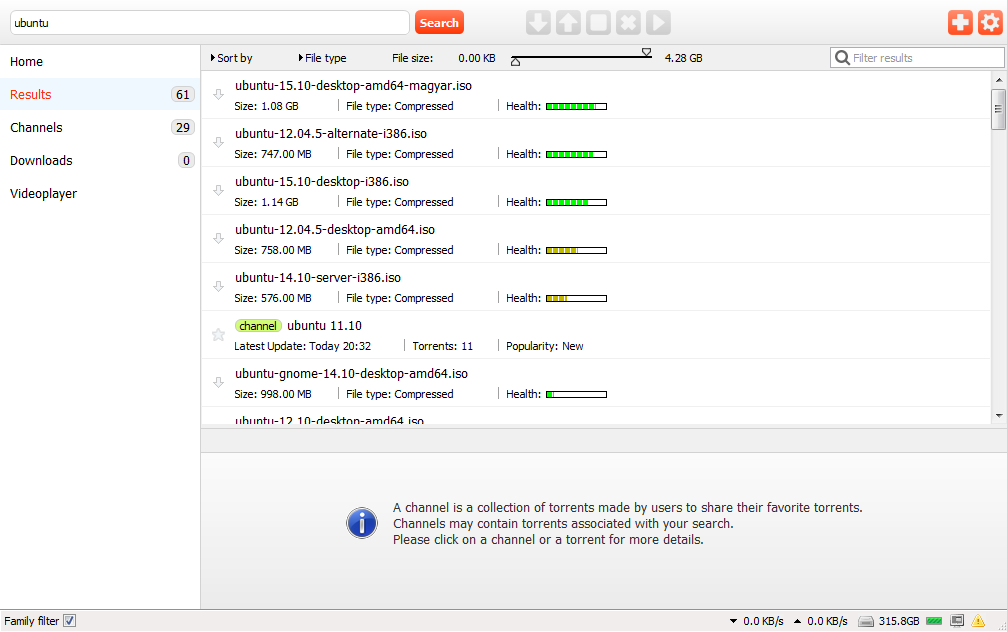
\includegraphics[width=\linewidth]{introduction/images/tribler_screenshot.png}
	\caption{Screenshot of Tribler v6.5.2.}
	\label{fig:tribler_screenshot}
\end{figure}


Tribler is a research platform for self organizing systems and online cooperation.
All research is embedded in the Tribler BitTorrent client, visible in Figure~\ref{fig:tribler_screenshot}.
Tribler can be downloaded free of charge from the Tribler website\footnote{\url{https://www.tribler.org}}.
It has been downloaded approximately 1.8 million times, has more than 2 thousand monthly active users and anticipating more growth in the near future.
This makes Tribler one of the few research projects that allow researchers to run experimental code \enquote{in the wild} on a large heterogeneous user group.

Tribler focuses on the following goals:
\begin{itemize}
    \item Allow for secure and private communication and sharing of data.
    \item Enforce user contribution in the network by making use of the Multi-Chain.
    \item Reward seeding of poorly-seeded content by using credit mining.
    \item Make it impossible to shut Tribler down, unless the Internet itself as a whole gets taken down.
\end{itemize}

A fully decentralized ecosystem i.e. no central components present, is Tribler's approach to achieve these goals.
Tribler has been designed and build with this focus~\cite{Pouwelse-tribler,Bakker-tribler} \todo{cites}.
A distributed network requires both the presence and collaboration of participants, called peers, to be able to achieve this.

\section{Dispersy}
The Distributed Permission System (Dispersy) is an elastic database system written in the Python programming language and uses SQLite as its underlying database engine.

\subsection{Challenging network conditions}
Nowadays almost all devices have an internet connection, often running in a challenged network environment \cite{dispersy2016dispersy}.
Challenging conditions can be found in many different networks such as Peer-to-Peer (P2P) networks or delay tolerant networks (DTNs).
The limitations of these networks are often low internet speed, connection drops, package loss and long communication delays.
P2P networks in particular create challenging conditions as many devices are not online at all times, they are often behind NAT-firewall constrained internet connections and one often interacts with byzantine peers.
Additionally, smartphones and other embedded devices such as Raspberry PI's often have less processing capacity or finite battery lifetime.

Dispersy is designed to still function when faced with these challenging network conditions.
It does this by using optimized algorithms, protocols and other techniques such as bloom filters to minimize the amount of resources needed.
By making use of strong elliptic curve cryptography, nodes are identified in a secure and anonymous way.

\subsection{Decentralized}
Dispersy is fully decentralized with the exception of bootstrap servers.
It can run on systems with a large number of nodes, without any sever architecture needed.
All nodes perform the same algorithmic procedures and tasks and do not differentiate between any node i.e. all nodes are equal.

Furthermore, Dispersy provides on-to-one and one-to-many data dissemination mechanisms to forward data to nodes.
Eventually, all data will reach all nodes in the network, overcoming challenging network conditions.

\section{BitTorrent protocol}
The BitTorrent protocol was introduced in 2001 and been a huge part of the internet ever since \cite{Cohen2001BitTorrent}.
Estimates as of 2009 indicate that 43\% to 70\% of all internet traffic world-wide is caused by peer-to-peer networks \cite{schulze2009internet}.
As of February 2013, BitTorrent was responsible for 3.35\% of all worldwide bandwidth \cite{palo2013application}, having 15 - 27 million concurrent users at any time \cite{wang2013measuring} and more than 150 million users in total \cite{reuters2012bittorrent}.

Downloading files is done in a decentralized way, that means no central entity such as a server is needed.
By obtaining a torrent file, users can download files associated with this torrent using a program that is compatible with the BitTorrent protocol.\\

A torrent is a file that contains meta information about the directories and files to be distributed.
More specifically, it contains names, sizes, hashes to verify the integrity of the files and the folder structure of the content to be downloaded.
A torrent usually contains a list of trackers and their network addresses.
These trackers help participants locate each other and form efficient distribution groups -- \emph{swarms}.
 

When sharing files by using the BitTorrent protocol, a user (or peer) that uploads i.e. allows other peers to download the user's files using the user's upload connection, is called a seeder.
A peer that is downloading a file of a seeder is called a leecher.
Any peer can be both a seeder and leecher at the same time, and join the network at any given time.\\

The ratio between the total data downloaded and uploaded is called the seeding ratio \cite{Cohen-bittorrent}.
The seeding ratio can be seen as an indication of the level of collaboration i.e. giving back resources to the network.\\

%Seeding can be seen as an interaction between peers, where the seeder aids the leeching peer.
%By utilizing the seeders upload bandwidth, the leeching peer can use his download bandwidth to download a file.
%While there is a clear incentive for the leecher by downloading the desired file, there is none for the seeder.
%Especially since the leecher has a little chance of becoming also be a seeder for the original seeder \cite{Lai-Incentives}.\\

%Having peers actively and persistently contribute to the network will increase the network's health which in turn provides several benefits for all peers.
%A more healthy network results in a higher availability of seeders and results in high download speeds.
%It has been shown that private communities i.e. "darknets" where the seeding ratio is high, provides better download conditions \cite{meulpolder-privatecommunities}.
%In these private communities, trackers i.e. central components introduce peers to each other using the Tit-for-tat approach \cite{cohen-titfortat}.
%The Tit-for-Tat approach is aiding peers who have aided you in the past,
%The absence of trackers, which is often the case in public networks, results in free-riding \cite{Adar-Freeriding}.
%A free-riding peer does not or gives little back to the network while receiving all benefits i.e. download without any restriction.
%\todo{Explain the optimistic chocking approach.}
%BitTorrent applies a variation of the Tit-for-tat strategy, optimistic chocking, to combat this problem.
%The Tit-for-Tat strategy is to only provide help to peers that return this help.
%However, it has been shown that this approach is not effective in battling abuse \cite{Pouwelse-tribler}.


\todo{more explanation?}
\section{Goal \& Outline}
In this thesis we introduce a performance regression testing system that makes use of benchmarking.
Whenever a codebase changes, it is important to measure the effects of these changes.
Negative changes can manifest themselves as reduced computational speed, increased memory consumption or reduced responsiveness of a program.
Each of these result in a reduction of user experience.
For instance, Google Chrome makes use of performance regression testing to gain insight into the effect of code changes.
While it is one of the fastest browsers currently available, it is also know for it's extreme RAM consumption which may lead to issues on older devices \cite{ram2012chrome}.

In this chapter we provided an introduction of this thesis and presented the research questions this thesis aims to answer. 
This section describes the other chapters in this thesis.
Chapter~\ref{chp:problem-description} provides the problem description and the research questions this thesis attempts to answer.
Chapter~\ref{cpt:related_work} presents related work on the subjects overlapping this thesis work.
Chapter~\ref{cpt:pythons_thread_model} explains the python threading module and why parallel programming in Python is different from a language such as Java. Additionally, the subjects of multi-threaded performance and asynchrony are covered.
Chapter~\ref{cpt:tribler_current_state} elaborates on I/O problem Tribler is currently facing and the current state.
Chapter~\ref{implementation_and_experiments} presents the implementation details and experimental results of this work.
Finally, Chapter~\ref{cpt:conclusion_and_future_work} concludes this thesis and provides future work.
